% Options for packages loaded elsewhere
% Options for packages loaded elsewhere
\PassOptionsToPackage{unicode}{hyperref}
\PassOptionsToPackage{hyphens}{url}
%
\documentclass[
  ignorenonframetext,
]{beamer}
\newif\ifbibliography
\usepackage{pgfpages}
\setbeamertemplate{caption}[numbered]
\setbeamertemplate{caption label separator}{: }
\setbeamercolor{caption name}{fg=normal text.fg}
\beamertemplatenavigationsymbolsempty
% remove section numbering
\setbeamertemplate{part page}{
  \centering
  \begin{beamercolorbox}[sep=16pt,center]{part title}
    \usebeamerfont{part title}\insertpart\par
  \end{beamercolorbox}
}
\setbeamertemplate{section page}{
  \centering
  \begin{beamercolorbox}[sep=12pt,center]{section title}
    \usebeamerfont{section title}\insertsection\par
  \end{beamercolorbox}
}
\setbeamertemplate{subsection page}{
  \centering
  \begin{beamercolorbox}[sep=8pt,center]{subsection title}
    \usebeamerfont{subsection title}\insertsubsection\par
  \end{beamercolorbox}
}
% Prevent slide breaks in the middle of a paragraph
\widowpenalties 1 10000
\raggedbottom
\AtBeginPart{
  \frame{\partpage}
}
\AtBeginSection{
  \ifbibliography
  \else
    \frame{\sectionpage}
  \fi
}
\AtBeginSubsection{
  \frame{\subsectionpage}
}
\usepackage{iftex}
\ifPDFTeX
  \usepackage[T1]{fontenc}
  \usepackage[utf8]{inputenc}
  \usepackage{textcomp} % provide euro and other symbols
\else % if luatex or xetex
  \usepackage{unicode-math} % this also loads fontspec
  \defaultfontfeatures{Scale=MatchLowercase}
  \defaultfontfeatures[\rmfamily]{Ligatures=TeX,Scale=1}
\fi
\usepackage{lmodern}

\ifPDFTeX\else
  % xetex/luatex font selection
\fi
% Use upquote if available, for straight quotes in verbatim environments
\IfFileExists{upquote.sty}{\usepackage{upquote}}{}
\IfFileExists{microtype.sty}{% use microtype if available
  \usepackage[]{microtype}
  \UseMicrotypeSet[protrusion]{basicmath} % disable protrusion for tt fonts
}{}
\makeatletter
\@ifundefined{KOMAClassName}{% if non-KOMA class
  \IfFileExists{parskip.sty}{%
    \usepackage{parskip}
  }{% else
    \setlength{\parindent}{0pt}
    \setlength{\parskip}{6pt plus 2pt minus 1pt}}
}{% if KOMA class
  \KOMAoptions{parskip=half}}
\makeatother


\usepackage{longtable,booktabs,array}
\usepackage{calc} % for calculating minipage widths
\usepackage{caption}
% Make caption package work with longtable
\makeatletter
\def\fnum@table{\tablename~\thetable}
\makeatother
\usepackage{graphicx}
\makeatletter
\newsavebox\pandoc@box
\newcommand*\pandocbounded[1]{% scales image to fit in text height/width
  \sbox\pandoc@box{#1}%
  \Gscale@div\@tempa{\textheight}{\dimexpr\ht\pandoc@box+\dp\pandoc@box\relax}%
  \Gscale@div\@tempb{\linewidth}{\wd\pandoc@box}%
  \ifdim\@tempb\p@<\@tempa\p@\let\@tempa\@tempb\fi% select the smaller of both
  \ifdim\@tempa\p@<\p@\scalebox{\@tempa}{\usebox\pandoc@box}%
  \else\usebox{\pandoc@box}%
  \fi%
}
% Set default figure placement to htbp
\def\fps@figure{htbp}
\makeatother





\setlength{\emergencystretch}{3em} % prevent overfull lines

\providecommand{\tightlist}{%
  \setlength{\itemsep}{0pt}\setlength{\parskip}{0pt}}



 


\makeatletter
\@ifpackageloaded{tcolorbox}{}{\usepackage[skins,breakable]{tcolorbox}}
\@ifpackageloaded{fontawesome5}{}{\usepackage{fontawesome5}}
\definecolor{quarto-callout-color}{HTML}{909090}
\definecolor{quarto-callout-note-color}{HTML}{0758E5}
\definecolor{quarto-callout-important-color}{HTML}{CC1914}
\definecolor{quarto-callout-warning-color}{HTML}{EB9113}
\definecolor{quarto-callout-tip-color}{HTML}{00A047}
\definecolor{quarto-callout-caution-color}{HTML}{FC5300}
\definecolor{quarto-callout-color-frame}{HTML}{acacac}
\definecolor{quarto-callout-note-color-frame}{HTML}{4582ec}
\definecolor{quarto-callout-important-color-frame}{HTML}{d9534f}
\definecolor{quarto-callout-warning-color-frame}{HTML}{f0ad4e}
\definecolor{quarto-callout-tip-color-frame}{HTML}{02b875}
\definecolor{quarto-callout-caution-color-frame}{HTML}{fd7e14}
\makeatother
\makeatletter
\@ifpackageloaded{caption}{}{\usepackage{caption}}
\AtBeginDocument{%
\ifdefined\contentsname
  \renewcommand*\contentsname{Table of contents}
\else
  \newcommand\contentsname{Table of contents}
\fi
\ifdefined\listfigurename
  \renewcommand*\listfigurename{List of Figures}
\else
  \newcommand\listfigurename{List of Figures}
\fi
\ifdefined\listtablename
  \renewcommand*\listtablename{List of Tables}
\else
  \newcommand\listtablename{List of Tables}
\fi
\ifdefined\figurename
  \renewcommand*\figurename{Figure}
\else
  \newcommand\figurename{Figure}
\fi
\ifdefined\tablename
  \renewcommand*\tablename{Table}
\else
  \newcommand\tablename{Table}
\fi
}
\@ifpackageloaded{float}{}{\usepackage{float}}
\floatstyle{ruled}
\@ifundefined{c@chapter}{\newfloat{codelisting}{h}{lop}}{\newfloat{codelisting}{h}{lop}[chapter]}
\floatname{codelisting}{Listing}
\newcommand*\listoflistings{\listof{codelisting}{List of Listings}}
\makeatother
\makeatletter
\makeatother
\makeatletter
\@ifpackageloaded{caption}{}{\usepackage{caption}}
\@ifpackageloaded{subcaption}{}{\usepackage{subcaption}}
\makeatother
\makeatletter
\@ifpackageloaded{fontawesome5}{}{\usepackage{fontawesome5}}
\makeatother

\usepackage{bookmark}
\IfFileExists{xurl.sty}{\usepackage{xurl}}{} % add URL line breaks if available
\urlstyle{same}
\hypersetup{
  pdftitle={SmartPolicy Recommender System},
  pdfauthor={Dr Patrick Altmeyer},
  hidelinks,
  pdfcreator={LaTeX via pandoc}}


\title{\textbf{SmartPolicy} Recommender System}
\subtitle{AI Risks, Mitigation and Maintenance}
\author{Dr Patrick Altmeyer}
\date{2026-03-27}
\institute{Delft University of Technology}

\begin{document}
\frame{\titlepage}


\section{Introduction}\label{introduction}

\begin{frame}{SmartPolicy}
\phantomsection\label{smartpolicy}
\begin{itemize}
\tightlist
\item
  \textbf{Goal}: recommender system (RS) for insurance policies

  \begin{itemize}
  \tightlist
  \item
    why? more tailored customer experience
  \end{itemize}
\item
  \textbf{How-to}: use granular data and expressive models to train RS

  \begin{itemize}
  \tightlist
  \item
    \emph{data} on demographics \faIcon{person} , prior claims
    \faIcon{file}, driving \faIcon{car}, health \faIcon{book-medical},
    home \faIcon{house}
  \item
    \emph{models} likely to include opaque machine learning
  \end{itemize}
\end{itemize}

\begin{tcolorbox}[enhanced jigsaw, coltitle=black, opacityback=0, toprule=.15mm, breakable, left=2mm, rightrule=.15mm, titlerule=0mm, colframe=quarto-callout-tip-color-frame, opacitybacktitle=0.6, bottomtitle=1mm, toptitle=1mm, bottomrule=.15mm, title=\textcolor{quarto-callout-tip-color}{\faLightbulb}\hspace{0.5em}{ERGO context}, arc=.35mm, leftrule=.75mm, colback=white, colbacktitle=quarto-callout-tip-color!10!white]

Pan-European insurer (Munich Re subsidiary), operating across EU, US,
and Asia

\end{tcolorbox}
\end{frame}

\begin{frame}{SmartPolicy}
\phantomsection\label{smartpolicy-1}
\begin{itemize}
\tightlist
\item
  \textbf{How-to}: use granular data and powerful models to train RS

  \begin{itemize}
  \tightlist
  \item
    all \emph{data} sources likely to include sensitive data

    \begin{itemize}
    \tightlist
    \item
      Applicable: \href{https://gdpr-info.eu/art-9-gdpr/}{GDPR Art. 9}
      (special categories),
      \href{https://gdpr-info.eu/art-22-gdpr/}{Art. 22} (automated
      decisions), \href{https://gdpr-info.eu/art-35-gdpr/}{Art. 35}
      (Data Protection Impact Assessment)
    \end{itemize}
  \item
    more powerful \emph{models} likely not explainable

    \begin{itemize}
    \tightlist
    \item
      Applicable:
      \href{https://eur-lex.europa.eu/legal-content/EN/TXT/?uri=CELEX:32024R1689}{EU
      AI Act} (high-risk obligations),
      \href{https://gdpr-info.eu/art-22-gdpr/}{GDPR Art. 22} (right to
      explanation)
    \end{itemize}
  \end{itemize}
\end{itemize}
\end{frame}

\section{Applicable Regulation}\label{applicable-regulation}

\begin{frame}{EU Regulation: AI Act}
\phantomsection\label{eu-regulation-ai-act}
\begin{itemize}
\tightlist
\item
  \href{https://artificialintelligenceact.eu/article/6/}{Article 6}
  (High-Risk AI Systems\footnote<.->[frame]{High-risk compliance
    deadline: \textbf{2 August 2026}})

  \begin{itemize}
  \tightlist
  \item
    ``{[}\ldots{]} AI system performs profiling of natural persons''
  \item
    ``AI systems for risk assessment and pricing in life and health
    insurance''---\href{https://artificialintelligenceact.eu/annex/3/}{Annex
    III §5(c)}
  \item
    all data sources (except \faIcon{house}) directly affected
  \end{itemize}
\item
  \href{https://artificialintelligenceact.eu/article/26/}{Article 26}
  (obligations): risk management system, data governance, technical
  documentation, human oversight, conformity assessment, registration in
  EU database.
\item
  \href{https://artificialintelligenceact.eu/article/27/}{Article 27}:
  Fundamental Rights Impact Assessment (FRIA) for High-Risk AI Systems
\end{itemize}
\end{frame}

\begin{frame}{EU Regulation: GDPR}
\phantomsection\label{eu-regulation-gdpr}
\begin{longtable}[]{@{}
  >{\raggedright\arraybackslash}p{(\linewidth - 2\tabcolsep) * \real{0.2571}}
  >{\raggedright\arraybackslash}p{(\linewidth - 2\tabcolsep) * \real{0.7429}}@{}}
\toprule\noalign{}
\begin{minipage}[b]{\linewidth}\raggedright
Article
\end{minipage} & \begin{minipage}[b]{\linewidth}\raggedright
Relevance to SmartPolicy
\end{minipage} \\
\midrule\noalign{}
\endhead
\href{https://gdpr-info.eu/art-5-gdpr/}{Art. 5} & \textbf{Data
minimisation}: collect only what is strictly necessary \\
\href{https://gdpr-info.eu/art-9-gdpr/}{Art. 9} & \textbf{Special
categories}: health, driving behaviour data require explicit consent or
legal basis \\
\href{https://gdpr-info.eu/art-22-gdpr/}{Art. 22} & \textbf{Automated
decisions}: right not to be subject to solely automated decisions with
significant effects; special-category data further restricted \\
\href{https://gdpr-info.eu/art-35-gdpr/}{Art. 35} & \textbf{DPIA
mandatory} when processing sensitive data at scale for profiling
(definitely \faIcon{book-medical}, \faIcon{person}) \\
\bottomrule\noalign{}
\end{longtable}
\end{frame}

\begin{frame}{Beyond EU: United States}
\phantomsection\label{beyond-eu-united-states}
\begin{itemize}
\tightlist
\item
  \textbf{USA}: No unified federal AI-in-insurance law; oversight is
  state-driven and fragmented

  \begin{itemize}
  \tightlist
  \item
    A \textbf{patchwork} of state rules creates compliance complexity
    for multi-state operations.
  \end{itemize}
\item
  \textbf{Asia}: country-specific and complex;
  \href{https://cms.law/en/int/expert-guides/ai-regulation-scanner/china}{China},
  for example, still lacks standalone, comprehensive statute.
\end{itemize}

\begin{tcolorbox}[enhanced jigsaw, coltitle=black, opacityback=0, toprule=.15mm, breakable, left=2mm, rightrule=.15mm, titlerule=0mm, colframe=quarto-callout-tip-color-frame, opacitybacktitle=0.6, bottomtitle=1mm, toptitle=1mm, bottomrule=.15mm, title=\textcolor{quarto-callout-tip-color}{\faLightbulb}\hspace{0.5em}{Tip}, arc=.35mm, leftrule=.75mm, colback=white, colbacktitle=quarto-callout-tip-color!10!white]

\textbf{Recommendation}: prioritise EU rollout first. The EU AI Act
provides a clear, comprehensive framework.

\end{tcolorbox}
\end{frame}

\section{AI-related Risks}\label{ai-related-risks}

\begin{frame}{Specific Risks: Data}
\phantomsection\label{specific-risks-data}
\begin{enumerate}
\tightlist
\item
  \textbf{Sensitive variables included directly}: \faIcon{book-medical}
  data (\href{https://gdpr-info.eu/art-9-gdpr/}{Art. 9} special
  category)
\item
  \textbf{Proxies of sensitive variables}: \faIcon{house} as proxy for
  ethnicity; \faIcon{person} may encode gender, religion, disability
\item
  \textbf{Historical bias}: past \faIcon{file} data likely reflects
  structural under/over-reporting by vulnerable groups
\item
  \textbf{Data minimisation violation}
  (\href{https://gdpr-info.eu/art-5-gdpr/}{GDPR Art. 5}): temptation to
  use all available data for data-hungry models
\end{enumerate}
\end{frame}

\begin{frame}{Specific Risks: Models}
\phantomsection\label{specific-risks-models}
\begin{enumerate}
\tightlist
\item
  \textbf{Opacity}: most competitive RS are inherently black-box ---
  violates \href{https://gdpr-info.eu/art-22-gdpr/}{GDPR Art. 22} right
  to explanation and
  \href{https://artificialintelligenceact.eu/high-level-summary/}{EU AI
  Act} transparency requirements.
\item
  \textbf{Historical bias}: models are representations of training data.
\item
  \textbf{Adversarial vulnerability}: e.g.~fake claim histories
  \faIcon{file}
\item
  \textbf{Data drift → model drift}: insurance risk profiles shift over
  time (e.g.~post-pandemic \faIcon{book-medical}, EV adoption for
  \faIcon{car}); models degrade silently without monitoring
\item
  \textbf{Membership inference attacks}: genuine privacy risk for
  sensitive \faIcon{book-medical}, \faIcon{person}, \faIcon{file}
\end{enumerate}
\end{frame}

\section{Mitigation Strategies}\label{mitigation-strategies}

\begin{frame}{Technical Mitigations: Opaque Models}
\phantomsection\label{technical-mitigations-opaque-models}
\begin{itemize}
\tightlist
\item
  \textbf{Start simple}: use interpretable models where feasible
  (e.g.~collaborative filtering; GAMs instead of DL; \ldots)
\item
  \textbf{Post-hoc explainability and recourse}: e.g.~counterfactual
  explanations \emph{``what would change my recommendation?''}
\item
  \textbf{Fairness-aware training}: adversarial debiasing and mitigation
  (\href{https://fairlearn.org/v0.13/user_guide/mitigation/adversarial.html}{Fairlearn},
  \href{https://holisticai.readthedocs.io/en/latest/getting_started/bias/mitigation/inprocessing/bc_adversarial_debiasing_adversarial_debiasing.html}{Holistic
  AI}), \href{https://arxiv.org/abs/2601.16205}{counterfactual
  training}, \ldots{}
\item
  \textbf{Human-in-the-loop} for high-stakes outputs (e.g.~refusal to
  recommend any policy)---required by
  \href{https://artificialintelligenceact.eu/article/14/}{EU AI Act Art.
  14}
\end{itemize}
\end{frame}

\begin{frame}{Technical Mitigations: Robustness}
\phantomsection\label{technical-mitigations-robustness}
\begin{itemize}
\tightlist
\item
  \textbf{Uncertainty quantification}: Bayesian or ensemble methods;
  conformal prediction.
\item
  \textbf{Adversarial training}: train on perturbed inputs and/or use
  data augmentation techniques (e.g.~counterfactuals)
\item
  \textbf{Drift detection}: monitor input/output distributions
\item
  \textbf{Regular retraining schedule}: define a model lifecycle policy
\end{itemize}
\end{frame}

\begin{frame}{Technical Mitigations: Data}
\phantomsection\label{technical-mitigations-data}
\begin{itemize}
\tightlist
\item
  \textbf{Data minimisation}
  (\href{https://gdpr-info.eu/art-25-gdpr/}{GDPR Art. 25}): define the
  minimal feature set for each insurance line before modelling
\item
  \textbf{Proxy audits}: test for and remove non-sensitive features
  correlated with sensitive features especially in
  \faIcon{book-medical}, \faIcon{person}, \faIcon{file} (use
  e.g.~\href{https://fairlearn.org/v0.13/user_guide/mitigation/preprocessing.html}{Fairlearn})
\end{itemize}
\end{frame}

\begin{frame}{Governance Mitigations: Data}
\phantomsection\label{governance-mitigations-data}
\begin{itemize}
\tightlist
\item
  \textbf{Data governance policy}: define data retention periods,
  deletion procedures, consent management
\item
  \textbf{Datasheets for Datasets}
  (\href{https://dl.acm.org/doi/10.1145/3458723}{Gebru et al., 2021}):
  clear guidelines for documenting training data (see
  \href{https://github.com/bridge2ai/data-sheets-schema}{FOSS
  implementation})
\item
  \textbf{Mandatory DPIA} before deployment
  (\href{https://gdpr-info.eu/art-35-gdpr/}{GDPR Art. 35}): purpose,
  legal basis, risks, and controls; update at each major model revision
  (definitely \faIcon{book-medical}, \faIcon{person}, likely all)
\end{itemize}
\end{frame}

\begin{frame}{Governance Mitigations: Models}
\phantomsection\label{governance-mitigations-models}
\begin{itemize}
\tightlist
\item
  \textbf{Model cards} (\href{https://arxiv.org/abs/1810.03993}{Mitchell
  et al., 2019, arXiv:1810.03993}: document model, intended use,
  limitations, training data, \ldots{}

  \begin{itemize}
  \tightlist
  \item
    Markdown with YAML as already standard practice on
    \href{https://huggingface.co/docs/hub/model-card-annotated}{HuggingFace}
  \end{itemize}
\item
  \textbf{Version control}: model and data linked on HF; consider
  semantic versioning
\item
  \textbf{Internal red-teaming}: structured adversarial testing sessions
  and hackathons
\end{itemize}
\end{frame}

\begin{frame}{Governance Mitigations: End-to-end}
\phantomsection\label{governance-mitigations-end-to-end}
End-to-end auditing framework as reference point:

\begin{figure}[H]

{\centering \pandocbounded{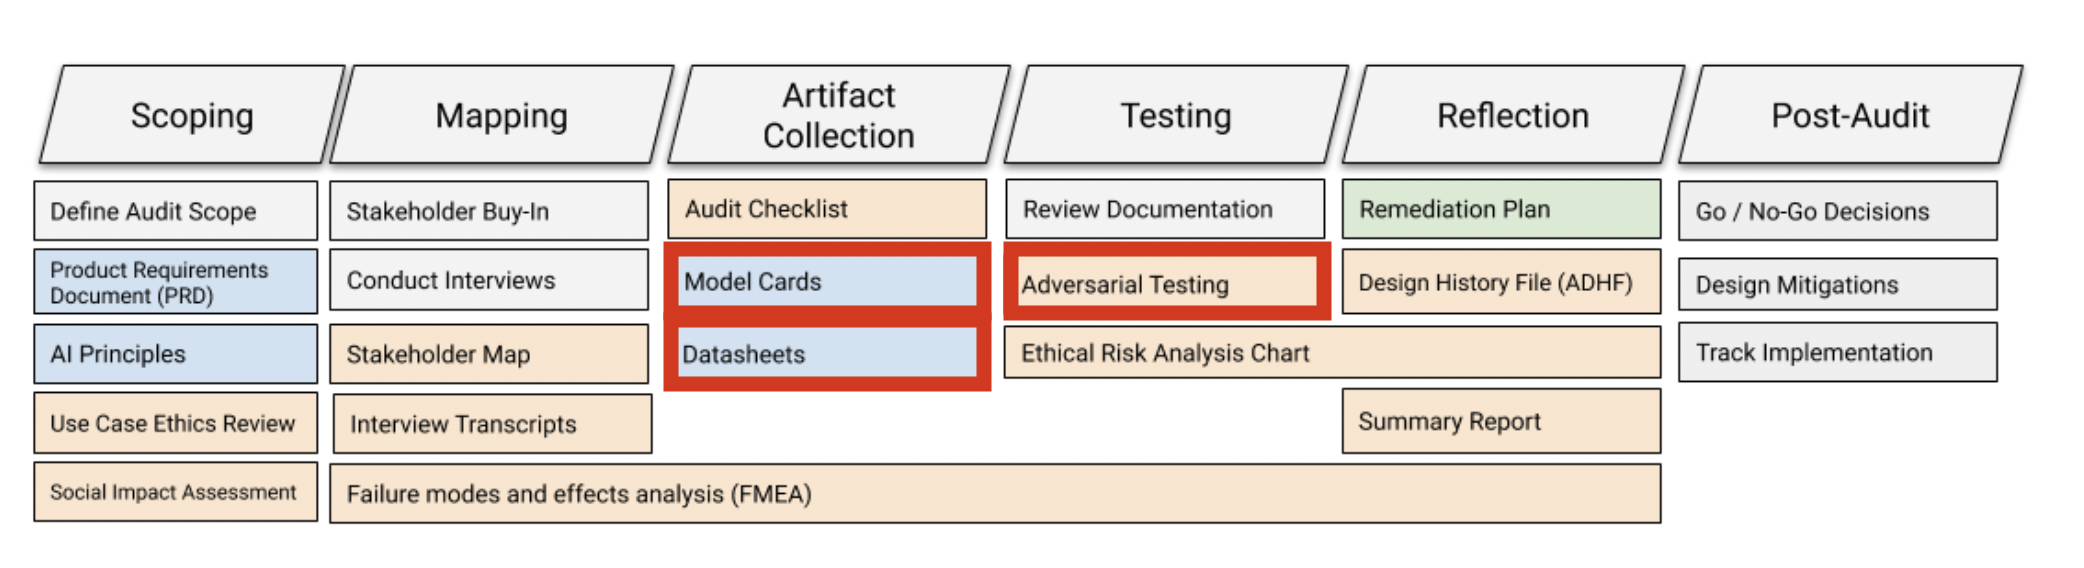
\includegraphics[keepaspectratio]{www/endtoend.png}}

}

\caption{\textbf{End-to-end algorithmic auditing}
(\href{https://arxiv.org/abs/2001.00973}{Raji et al., @ FA(Cc)T* '20,
arXiv:2001.00973}): structured audits at every stage of the development
lifecycle (scoping → mapping → artefact collection → testing →
reflection).}

\end{figure}%
\end{frame}

\begin{frame}{Governance Mitigations --- Open Source Considerations}
\phantomsection\label{governance-mitigations-open-source-considerations}
\begin{itemize}
\tightlist
\item
  Selectively \textbf{open-sourcing code and models} can generate
  external scrutiny, bug reports, and reputational goodwill
\item
  Open-source \emph{models} carry \textbf{inherent risks}: membership
  inference attacks become easier
\end{itemize}

\begin{tcolorbox}[enhanced jigsaw, coltitle=black, opacityback=0, toprule=.15mm, breakable, left=2mm, rightrule=.15mm, titlerule=0mm, colframe=quarto-callout-tip-color-frame, opacitybacktitle=0.6, bottomtitle=1mm, toptitle=1mm, bottomrule=.15mm, title=\textcolor{quarto-callout-tip-color}{\faLightbulb}\hspace{0.5em}{FOSS Practices}, arc=.35mm, leftrule=.75mm, colback=white, colbacktitle=quarto-callout-tip-color!10!white]

In the FOSS space, essentially all code is treated \textbf{packages}
(facilitates usage, extensibility, \ldots)

\end{tcolorbox}
\end{frame}

\section{Documentation}\label{documentation}

\begin{frame}{Key Documents\footnote<.->[frame]{Mandatory \textbf{DPIA}
  and \textbf{FRIA} ommitted from table.}}
\phantomsection\label{key-documents}
\begin{longtable}[]{@{}
  >{\raggedright\arraybackslash}p{(\linewidth - 4\tabcolsep) * \real{0.3333}}
  >{\raggedright\arraybackslash}p{(\linewidth - 4\tabcolsep) * \real{0.3333}}
  >{\raggedright\arraybackslash}p{(\linewidth - 4\tabcolsep) * \real{0.3333}}@{}}
\toprule\noalign{}
\begin{minipage}[b]{\linewidth}\raggedright
Document
\end{minipage} & \begin{minipage}[b]{\linewidth}\raggedright
Trigger
\end{minipage} & \begin{minipage}[b]{\linewidth}\raggedright
\end{minipage} \\
\midrule\noalign{}
\endhead
\textbf{Datasheets} (\href{https://dl.acm.org/doi/10.1145/3458723}{Gebru
et al., 2021}) & Per training dataset & \\
\textbf{Model cards} (\href{https://arxiv.org/abs/1810.03993}{Mitchell
et al., 2019}) & Per model release & \\
\textbf{Technical documentation}
(\href{https://artificialintelligenceact.eu/article/11/}{EU AI Act Art.
11}) & commit; PR; release & \\
\bottomrule\noalign{}
\end{longtable}
\end{frame}

\begin{frame}{Notes on Technical Documentation}
\phantomsection\label{notes-on-technical-documentation}
\begin{itemize}
\tightlist
\item
  Treating all code as packages facilitates proper technical
  documentation standards.
\item
  Language-specific support is well-established
  (e.g.~\href{https://www.taija.org/CounterfactualExplanations.jl/stable/}{Julia}).
\item
  Rely on \textbf{Markdown} (README.md, CHANGELOG.md, \ldots) for
  version-controlled documentation.

  \begin{itemize}
  \tightlist
  \item
    Easily ingested by \href{https://quarto.org/}{Quarto} for publishing
    polished outputs
  \item
    Ideal for providing context to LLMs/agents.
  \end{itemize}
\end{itemize}
\end{frame}

\begin{frame}{Target Audience --- Internal}
\phantomsection\label{target-audience-internal}
\begin{itemize}
\tightlist
\item
  \textbf{Data scientists and ML engineers}: model cards, datasheets,
  technical documentation, version-controlled code and experiment logs.
\item
  \textbf{Customer-facing staff}: must be able to explain any
  recommendation and handle contestation
  (\href{https://artificialintelligenceact.eu/article/14/}{EU AI Act
  Art. 14}, \href{https://gdpr-info.eu/art-22-gdpr/}{GDPR Art. 22(3)})
\item
  \textbf{Compliance and legal}: DPIA, FRIA, \ldots{}
\item
  \textbf{Management}: use Quarto to go from Markdown to PDF, HTML,
  websites, presentations
  (\href{https://github.com/pat-alt/quarto-ergo}{like this one!}),
  \ldots{}
\end{itemize}
\end{frame}

\begin{frame}{Target Audience --- External}
\phantomsection\label{target-audience-external}
\begin{itemize}
\tightlist
\item
  \textbf{Regulators} (BaFin, national DPAs, EIOPA): technical
  documentation, DPIA, FRIA, conformity assessment records --- subject
  to inspection under
  \href{https://artificialintelligenceact.eu/article/74/}{EU AI Act Art.
  74}
\item
  \textbf{Customers}: simplified explanation notices (why was this
  policy recommended?); right to contest automated decisions
  (\href{https://gdpr-info.eu/art-22-gdpr/}{GDPR Art. 22}); privacy
  notice under \href{https://gdpr-info.eu/art-13-gdpr/}{GDPR Art. 13}
\item
  \textbf{Open-source community} (if applicable): public model cards,
  fairness evaluation results, code documentation --- supports external
  red-teaming and transparency signalling
\end{itemize}
\end{frame}

\begin{frame}{Keeping Documentation Up-to-Date}
\phantomsection\label{keeping-documentation-up-to-date}
\begin{itemize}
\tightlist
\item
  If above is properly implemented, state of documentation will always
  be consistent with the state of:

  \begin{enumerate}
  \tightlist
  \item
    Data (datasheets)
  \item
    Models (model cards)
  \item
    Code (technical docs)
  \end{enumerate}
\item
  Recommending HuggingFace for 1-2, GitHub/Gitlab for 3.
\end{itemize}
\end{frame}

\section{Questions?}\label{questions}




\end{document}
